\chapter{Shortest Paths}
Ajur had found a map of the cemetery. He used it to try to find the best way to go to the water fountain. Then he remembered his recent discussions with Rishnak and excitedly told Jura that by using graph theory methods, they would be able to find a path and maybe even the shortest path to the water fountain.

Rishnak overheard Ajur and realized that a good discussion of paths and shortest paths would be an ideal topic to pursue next.

Rishnak said, ``Consider a graph\footnote{For spanning trees, we consider only undirected graphs; however, for shortest paths we can consider both undirected and directed graphs.} in which you wish to find the shortest path from a specified source vertex to a specified destination vertex. Let's look at this familiar graph.''---Rishnak waved his hands and an undirected graph appeared in front of Ajur [Figure~\ref{12g1}]---``What's the shortest path from vertex~1 to vertex~6?''

\begin{figure}
\begin{center}
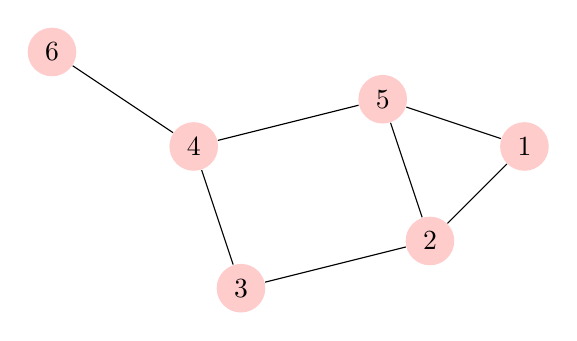
\begin{tikzpicture}
  [scale=.6,auto=left,every node/.style={circle,fill=red!20}]
  \node (n6) at (1,10) {6};
  \node (n4) at (4,8)  {4};
  \node (n5) at (8,9)  {5};
  \node (n1) at (11,8) {1};
  \node (n2) at (9,6)  {2};
  \node (n3) at (5,5)  {3};

  \foreach \from/\to in {n6/n4,n4/n5,n5/n1,n1/n2,n2/n5,n2/n3,n3/n4}
    \draw (\from) -- (\to);

\end{tikzpicture}
\caption{Example undirected graph for which we want to find the shortest path from vertex~1 to vertex~6}\label{12g1}
\end{center}
\end{figure}

Ajur jumped up with excitement and said he could easily draw the shortest path from source vertex~1 to destination vertex~6. He grabbed a stick and drew the graph in the dirt, then he showed the shortest path by thickening edges~$(1,5)$, $(5,4)$, and~$(4,6)$ [Figure~\ref{12g2}].

\begin{figure}
\begin{center}
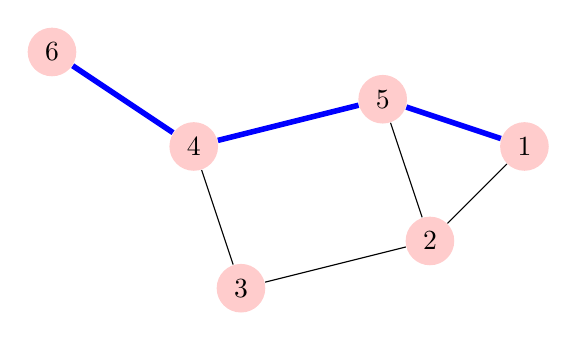
\begin{tikzpicture}
  [scale=.6,auto=left,every node/.style={circle,fill=red!20}]
  \node (n6) at (1,10) {6};
  \node (n4) at (4,8)  {4};
  \node (n5) at (8,9)  {5};
  \node (n1) at (11,8) {1};
  \node (n2) at (9,6)  {2};
  \node (n3) at (5,5)  {3};

  \foreach \from/\to in {n6/n4,n4/n5,n5/n1}
    \draw [line width=2 pt,color=blue] (\from) -- (\to);
\foreach \from/\to in {n3/n4,n3/n2,n2/n1,n2/n5}
    \draw  (\from) -- (\to);

\end{tikzpicture}
\caption{The graph from Figure~\ref{12g1} with the shortest Path (of length~3) shown from vertex~1 to vertex~6 using thick lines}\label{12g2}
\end{center}
\end{figure}

Pleased with Ajur's enthusiasm, Rishnak wanted to make sure that Ajur understood a general method for finding the shortest path from a source vertex to a destination vertex in any graph.

Rishnak said, ``Remember how to find a spanning tree for a given graph?''

Ajur said, ``Sure, yes.''

Rishnak said, ``Good. We can come up with a similar algorithm for finding the shortest path from a source vertex to a destination vertex, but first, we need to define distance \textbf{dist} of a vertex~$y$ as the number of vertices we must visit to get from the source vertex to vertex~$y$. We also define parent~\textbf{p} of a vertex as the parent vertex\footnote{You can also think of this as the \textit{previous} vertex.} that led us to vertex~$y$. Given these definitions, here is the algorithm:
\begin{enumerate}
\item Set \textbf{dist} for the source vertex to~0 (since the distance from the source vertex to itself is zero). Also set~\textbf{p} as being undefined.
\item Set both \textbf{dist} and~\textbf{p} for all other vertices as being undefined.
\item We start from the source vertex, so add that vertex to a queue.\footnote{In a queue, we can only add elements to the end and remove elements from the front, just like waiting in line at a grocery store. We can also inspect elements in the queue without changing their order.}
\item Remove the vertex from the front of the queue, calling this vertex~$w$. Find all vertices with undefined \textbf{dist} values that are adjacent to~$w$ and put them in set~$A$. Set \textbf{dist} for all of these vertices to be one more than the \textbf{dist} value for~$w$; also set~\textbf{p} to be vertex~$w$. Finally, add all vertices from set~$A$ to the queue.
\item Repeat Step~4 until the destination vertex has its \textbf{dist} value changed, meaning our algorithm has reached the destination vertex. We can then trace the shortest path back to the source vertex by following the~\textbf{p} vertices until we reach the source vertex.''
\end{enumerate}

Ajur knew this was a lot to try to understand. He used the example graph still in front of him [Figure~\ref{12g1}], tracing the algorithm from source vertex~1. He said, ``Okay, so we start by letting the distance \textbf{dist} of vertex~1 be~0, then we add vertex~1 to the queue. We remove vertex~1 from the queue. It has adjacent vertices~2 and~5, so the \textbf{dist} values of these vertices are both set to~2. And vertices~2 and~5 are added to the queue, say with vertex~2 at the end of the queue. Also, the parent~\textbf{p} vertices of vertices~2 and~5 are both set to vertex~1.''

Rishnak said, ``Correct. Keep going.''

Ajur went on, ``Next, we remove vertex~5 from the queue. The only adjacent vertex with an undefined \textbf{dist} value is vertex~4, so we add it to the end of the queue. And we set the \textbf{dist} of vertex~4 to be~2 and the parent~\textbf{p} of vertex~4 to be vertex~5.''

Ajur thought for a moment, then said, ``The first element of the queue is now vertex~2, which we remove next. Next, we add the only adjacent vertex---vertex~3---to the queue. For vertex~3, we set \textbf{dist} to~2 (because it is one more than the \textbf(dist) value of vertex~2) and the parent \textbf{p} to vertex~2. Finally, we remove vertex~4 from the queue and therefore reach vertex~6, which we add to the queue. We set the \textbf{dist} of vertex~6 to be~3 and its parent \textbf{p} to vertex~4. And since vertex~6 is the destination vertex, we're done. The distance from vertex~1 to vertex~6 is~3, and we can work backwards to determine the path since \textbf{p}$(6)=4$, \textbf{p}$(4)=5$, and~\textbf{p}$(5)=1$, which is the source vertex.''

Ajur marveled at the systematic procedure that could be applied to any graph. He also realized that this procedure could be used to find the shortest path from a single source to all other vertices in a given graph. As he thought about this further, he said, ``And we could use this same algorithm to find the shortest paths between every pair of vertices in a graph.''

Rishnak smiled and said, ``There is a graph parameter called the \textit{diameter} of a graph. The diameter is the longest path from among the shortest paths between every pair of vertices. For the example graph we have been using [Figure~\ref{12g1}], the diameter is~3 since the shortest paths between every pair of vertices are of lengths~1, 2, and~3.''

Ajur nodded.

Rishnak flashed his hands and the original graph morphed into a new graph with two fewer edges [Figure~\ref{12g3}].  He said, ``Find the diameter of this graph, Ajur.''

\begin{figure}
\begin{center}
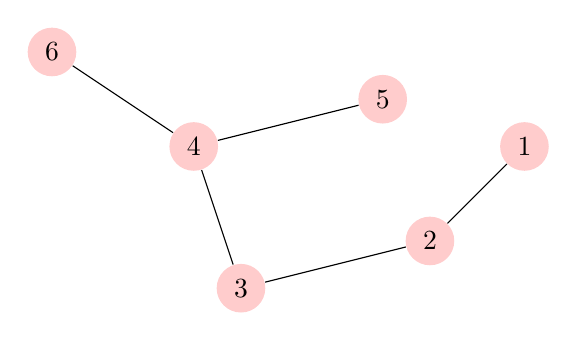
\begin{tikzpicture}
  [scale=.6,auto=left,every node/.style={circle,fill=red!20}]
  \node (n6) at (1,10) {6};
  \node (n4) at (4,8)  {4};
  \node (n5) at (8,9)  {5};
  \node (n1) at (11,8) {1};
  \node (n2) at (9,6)  {2};
  \node (n3) at (5,5)  {3};
   
  \foreach \from/\to in {n6/n4,n4/n5,n1/n2,n2/n3,n3/n4}
    \draw (\from) -- (\to);

\end{tikzpicture}
\caption{An example graph for which we wish to find the diameter}\label{12g3}
\end{center}
\end{figure}

Ajur studied the graph and said, ``Okay, this is the same graph but without edges~$(1,5)$ and~$(2,5)$. I see that this graph is a tree since there are no cycles in the graph. The longest path among all of the shortest paths is from vertex~1 to vertex~5---no wait, there's also a longest path from vertex~1 to vertex~6. Both of them are of length~4, so that's the diameter of this graph.  And therefore, there can be more than one path representing the diameter.''

Rishnak nodded and said, ``Correct. In general, a simple path with~$n$ vertices''---he waved his hands and a new graph appeared [Figure~\ref{12g4}]---``will have a diameter of~$n-1$. And for a complete graph\footnote{Remember that in a complete graph, there is an edge between every pair of vertices.} with~$n$ vertices, the diameter is always~$1$, as the shortest path between every pair of vertices is~$1$.''

Ajur again nodded.

Rishnak asked Ajur, ``Can you construct graphs, all with~$n$ vertices, that have diameters~$n-1,n-2,\ldots,2,\text{ and }1$?''

Ajur thought about this for a few moments. He said, ``Yes, that's not too hard. We already have the graph with a diameter of~$n-1$. Here's a graph with a diameter of~$n-2$''---he drew a graph in the dirt [Figure~\ref{12g5}]---``and another with diameter~$2$.''---he quickly drew another graph [Figure~\ref{12g6}].

Ajur smiled broadly and said, ``From these two graphs, you can infer the rest!''

\begin{figure}
\begin{center}
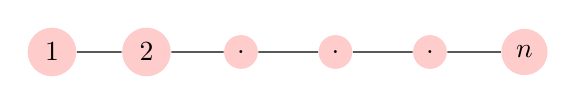
\begin{tikzpicture}
  [scale=.6,auto=left,every node/.style={circle,fill=red!20}]
  \node (n1) at (1,8) {$1$};
  \node (n2) at (3,8)  {$2$};
  \node (n3) at (5,8)  {$.$};
  \node (n4) at (7,8) {$.$};
  \node (n5) at (9,8)  {$.$};
  \node (n6) at (11,8)  {$n$};
   
  \foreach \from/\to in {n1/n2,n2/n3,n3/n4,n4/n5,n5/n6}
    \draw (\from) -- (\to);

\end{tikzpicture}
\caption{A graph with~$n$ vertices will always have a diameter of~$n-1$}\label{12g4}
\end{center}
\end{figure}

\begin{figure}
\begin{center}
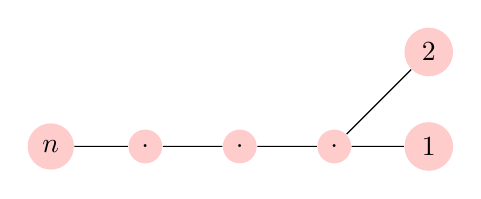
\begin{tikzpicture}
  [scale=.6,auto=left,every node/.style={circle,fill=red!20}]
  \node (n1) at (1,8) {$n$};
  \node (n2) at (3,8)  {$.$};
  \node (n3) at (5,8)  {$.$};
  \node (n4) at (7,8) {$.$};
  \node (n5) at (9,10)  {2};
  \node (n6) at (9,8)  {1};
   
  \foreach \from/\to in {n1/n2,n2/n3,n3/n4,n4/n5,n4/n6}
    \draw (\from) -- (\to);

\end{tikzpicture}
\caption{A graph with~$n$ vertices with a diameter of~$n-2$}\label{12g5}
\end{center}
\end{figure}
\begin{figure}
 \begin{center}
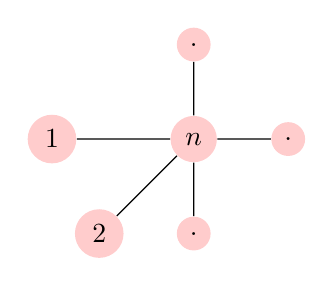
\begin{tikzpicture}
  [scale=.6,auto=left,every node/.style={circle,fill=red!20}]
  \node (n1) at (1,8) {$n$};
  \node (n2) at (1,10)  {$.$};
  \node (n3) at (3,8)  {$.$};
  \node (n4) at (1,6) {$.$};
  \node (n5) at (-1,6)  {2};
  \node (n6) at (-2,8)  {1};
   
  \foreach \from/\to in {n1/n2,n1/n3,n1/n4,n1/n5,n1/n6}
    \draw (\from) -- (\to);

\end{tikzpicture}
\caption{A graph with~$n$ vertices with a diameter of~$2$}\label{12g6}
\end{center}
\end{figure}

Rishnak said, ``Here is another interesting problem. Can we construct a regular undirected graph with given diameter~$k$?''

Ajur shrugged his shoulders and said, ``But how many vertices?''

Rishnak smiled as he continued, ``Yes, Ajur, an answer here is a set of graphs called \textit{Moore} graphs. In addition to diameter~$k$, we define degree~$d$ for the graph, meaning that each vertex has degree~$d$. Then we can calculate the number of vertices in the graph using this formula.''

Rishnak flashed his hands and the following formula appeared in the air in front of Ajur:
$$\text{number of vertices} = 1+\sum_{i=1}^{k-1} (d-1)^i$$

Ajur frowned as he studied the formula.

Rishnak said, ``Let me explain. We can understood this formula by drawing a graph in the shape of a rooted tree of depth~$k-1$''---Rishnak waved his hands and a new graph appeared [Figure~\ref{12g7}]---``which we have already seen.\footnote{This is the Petersen graph from Figure~\ref{5g4}.} In this graph, the root vertex has~$d$ children and every other vertex has~$d-1$ children. All of the leaf vertices break the tree properties since they are connected in such a way that every vertex has degree~$d$.''

Ajur studied this graph and said, ``Aha, and this graph's diameter is~$k$.''

Rishnak smiled and said, ``Precisely.''

\begin{figure}
\begin{center}
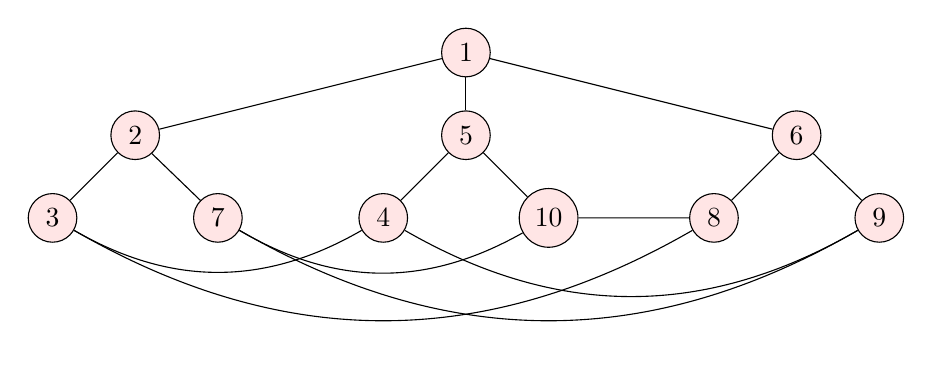
\begin{tikzpicture}[scale=0.7, every node/.style={circle,fill=red!10},level/.style={sibling distance=60mm/#1}]
\node [circle,draw] (z){$1$}
  child {node [circle,draw] (a) {$2$}
    child {node [circle,draw] (b) {$3$}}
    child {node [circle,draw] (c) {$7$}}}
    child {node [circle,draw] (d) {$5$}
        child {node [circle,draw] (e) {$4$}}
        child {node [circle,draw] (f) {$10$}}}
    child {node [circle,draw] (g) {$6$}
        child {node [circle,draw] (h) {$8$}}
        child {node [circle,draw] (i) {$9$}}};
\path
(b) edge [bend right] (h)
(b) edge [bend right] (e)
(c) edge [bend right] (i)
(c) edge [bend right] (f)
(e) edge [bend right] (i)
(f) edge (h)
;
\end{tikzpicture}
\caption{The Petersen graph from Figure~\ref{5g4} drawn in the shape of a rooted tree with a diameter of~$2$ and a degree of~$3$}\label{12g7}
\end{center}
\end{figure}

Ajur thought for a few moments, wondering about weighted graphs.  He said, ``Is there an algorithm to find shortest paths in weighted graphs?\footnote{Remember a weighted graph is a graph with weights or costs associated with each edge.}

Rishnak said, ``Yes, Ajur, good thinking.''  Rishnak waved his hands and a weighted graph appeared in the air [Figure~\ref{12g8}].

Rishnak continued, ``We can modify the shortest path algorithm from earlier to work for weighted graphs. Remember from that algorithm that we aim to find the shortest path from a source vertex to a destination vertex.  Then we redefine distance \textbf{dist} of a vertex~$y$ as the minimum sum of the weights along the edges we used to get from the source vertex to vertex~$y$. We still have parent~\textbf{p} of a vertex as the parent vertex that led us to vertex~$y$. Given these revised definitions, here is the algorithm:
\begin{enumerate}
\item Set \textbf{dist} for the source vertex to~0 (since the distance from the source vertex to itself is zero). Also set~\textbf{p} as being undefined.  Further, set \textbf{explored} to~$1$.
\item For all other vertices, set \textbf{dist} to~$\infty$, set \textbf{explored} to~$0$, and set~\textbf{p} as being undefined.
\item We start from the source vertex, so add that vertex to a queue.
\item Remove the vertex from the front of the queue, calling this vertex~$w$. Find all vertices with \textbf{explored} set to~$0$ that are adjacent to~$w$ and put them in set~$A$. For each vertex~$v\in A$, set its \textbf{dist} value to the minimum of the \textbf{dist} value for~$v$ and the sum of the \textbf{dist} value for~$w$ plus the weight of edge~$(w,v)$. If we use the sum here, then also set~\textbf{p} for vertex~$v$ to be~$w$ (since we found a shorter path).
\item Add the vertex with the smallest \textbf{dist} value from set~$A$ to the queue, also setting its \textbf{explored} value to~$1$.
\item Repeat Steps~4 and~5 until the destination vertex has its \textbf{dist} value changed, meaning our algorithm has reached the destination vertex. We can then trace the shortest path back to the source vertex by following the~\textbf{p} vertices until we reach the source vertex.''
\end{enumerate}


\begin{figure}
\begin{center}
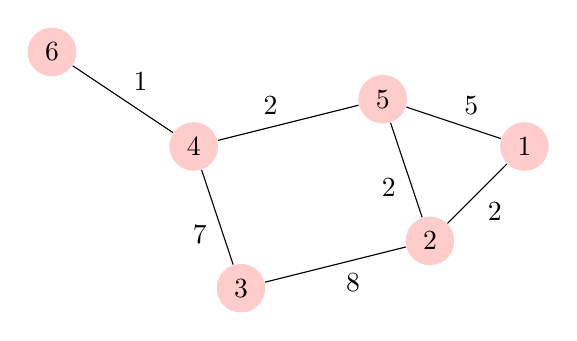
\begin{tikzpicture}
  [scale=.6,auto=left,every node/.style={circle,fill=red!20}]
  \tikzstyle{weight} = [fill=none]
  \node (n6) at (1,10) {6};
  \node (n4) at (4,8)  {4};
  \node (n5) at (8,9)  {5};
  \node (n1) at (11,8) {1};
  \node (n2) at (9,6)  {2};
  \node (n3) at (5,5)  {3};
  \foreach \source /\dest /\weight in {n6/n4/1,n4/n5/2,n5/n1/5,n1/n2/2,n2/n5/2,n2/n3/8,n3/n4/7} 
   \draw (\source) --node[weight] {$\weight$}  (\dest);
\foreach \source /\dest /\weight in {1/3/1} place \weight above of=\path;
  
  \end{tikzpicture}
\caption{A weighted graph with six vertices and seven edges for which we wish to find the shortest path from vertex~1 to vertex~6}\label{12g8}
\end{center}
\end{figure}

Ajur studied the graph in front of him, then drew it in the dirt.  He said, ``Okay, let me try to use the algorithm on this graph. Initially, \textbf{dist} of vertex~1 is set to~$0$, and for the rest of the vertices, \textbf{dist} is set to~$\infty$. Also, \textbf{explore} of vertex~1 is~$1$ since we have explored that vertex and~$0$ for the rest of the vertices. Scanning from vertex~1, \textbf{dist} of vertex~5 is~5 and \textbf{dist} of vertex~2 is~2. So the \textbf{p} labels of vertices~2 and~5 are both set to refer back to vertex~$1$.''

Rishnak said, ``Good, Ajur, that is a good start, yes.''

Ajur continued, ``Then we have to choose which vertex to explore next by selecting the adjacent vertex with the smallest \textbf{dist} value. That would be vertex~2, so we set \textbf{explore} for vertex~2 to~1. Next, we update \textbf{dist} of vertex~5 to~4 (since the sum~$2+2$ is less than~5) and \textbf{dist} of vertex~3 to~10. We also set their \textbf{p} values to both be vertex~2. We then select vertex~5 and set its \textbf{explore} value to~1. From vertex~5, \textbf{dist} of vertex~4 is set to~6 and its parent label is set to vertex~5.''---Ajur sighed as this was getting quite tedious---``Okay, then we go to vertex~4 so we set its \textbf{explore} label to~1. From vertex~4, \textbf{dist} of vertex~6 becomes 7 and its \textbf{p} value refers to vertex~4. In this case, \textbf{dist} of vertex~3 does not change. So finally, we set \textbf{explore} of vertex~6 to~1 and since it is the destination vertex, the algorithm stops.''

Ajur stepped back and looked again at the graph he had drawn [Figure~\ref{12g9}].  He said, ``We then know that the shortest path from vertex~1 to vertex~6 is of length~7. The path can be traced backward from vertex~6 through the \textbf{p} values, so we have \textbf{p}$(6)=4$, \textbf{p}$(4)=5$, \textbf{p}$(5)=2$, and~\textbf{p}$(2)=1$, the source vertex.''

\begin{figure}
\begin{center}
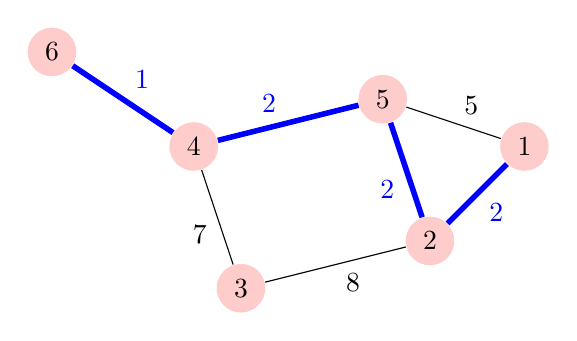
\begin{tikzpicture}
  [scale=.6,auto=left,every node/.style={circle,fill=red!20}]
  \tikzstyle{weight} = [fill=none]
  \node (n6) at (1,10) {6};
  \node (n4) at (4,8)  {4};
  \node (n5) at (8,9)  {5};
  \node (n1) at (11,8) {1};
  \node (n2) at (9,6)  {2};
  \node (n3) at (5,5)  {3};
  \foreach \source /\dest /\weight in {n5/n1/5,n2/n3/8,n3/n4/7} 
   \draw (\source) --node[weight] {$\weight$}  (\dest);
\foreach \source /\dest /\weight in {1/3/1} place \weight above of=\path;
  \foreach \source /\dest /\weight in {n6/n4/1,n4/n5/2,n1/n2/2,n2/n5/2} 
   \draw[line width=2 pt,color=blue] (\source) --node[weight] {$\weight$}  (\dest); 
  \end{tikzpicture}
\caption{The weighted graph from Figure~\ref{12g8} with the shortest path from vertex~1 to vertex~6 shown using thick lines}\label{12g9}
\end{center}
\end{figure}

Rishnak smiled as Ajur appreciated the power of the algorithm, knowing now that he could use this algorithm to compute the shortest route from the cemetery entrance to the water fountain---or anywhere else!

\subsection*{Question for the tenth day}
Rishnak said, ``It is now time for the question for the tenth day, Ajur. There are two parts to this question. Using the graph you have just seen [Figure~\ref{12g9}], first, how can you change the weight of a single edge such that the shortest path from vertex~1 to vertex~6 must go through vertex~3? Second, what is the minimum edge weight for the changed edge to still have the shortest path go through vertex~3?''

\textit{Before you turn the page, try to come up with answers of your own!}

\newpage
\subsection*{Answer for the tenth day}
Ajur thought about changing an edge incident on vertex~1 but quickly found that the shortest path would then simply follow the other vertex (i.e.,~vertex~2 or vertex~5).
After a few moments of pondering, Ajur erased the edge weight for edge~$(5,4)$ and replaced it with a new edge weight of~1000.

Ajur said, ``If the weight of edge~$(5,4)$ is increased to 1000, then the shortest path is forced to go through vertex~3.'' He drew the new shortest path using thick lines to emphasize the path [Figure~\ref{12qa1}].

Rishnak said, ``Good, and what could the minimum edge weight be for edge~$(5,4)$ to still have the shortest path go through vertex~3?''

Ajur said quickly, ``Easy, the shortest path through vertex~3 has a length of~18, so edge~$(5,4)$ would need to have a weight of~14 for the second-shortest path to be~19.''

\begin{figure}
\begin{center}
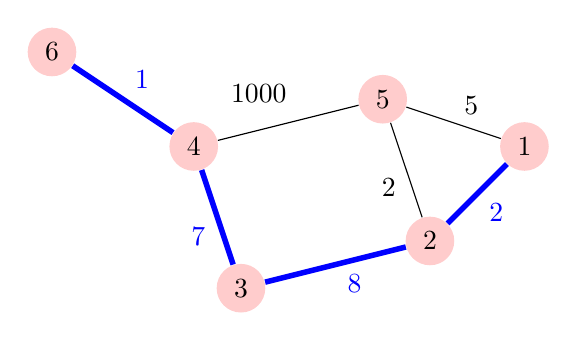
\begin{tikzpicture}
  [scale=.6,auto=left,every node/.style={circle,fill=red!20}]
  \tikzstyle{weight} = [fill=none]
  \node (n6) at (1,10) {6};
  \node (n4) at (4,8)  {4};
  \node (n5) at (8,9)  {5};
  \node (n1) at (11,8) {1};
  \node (n2) at (9,6)  {2};
  \node (n3) at (5,5)  {3};
  \foreach \source /\dest /\weight in {n5/n1/5,n2/n5/2,n4/n5/1000} 
   \draw (\source) --node[weight] {$\weight$}  (\dest);
\foreach \source /\dest /\weight in {1/3/1} place \weight above of=\path;
  \foreach \source /\dest /\weight in {n6/n4/1,n3/n4/7,n2/n3/8,n1/n2/2} 
   \draw[line width=2 pt,color=blue] (\source) --node[weight] {$\weight$}  (\dest); 
  \end{tikzpicture}
\caption{The weighted graph from Figure~\ref{12g8} with the shortest path from vertex~1 to vertex~6 shown using thick lines, this time going through vertex~3 given the increased edge weight of edge~$(5,4)$}\label{12qa1}
\end{center}
\end{figure}

Rishnak smiled and said, ``Yes, Ajur, very good.''

Ajur wanted to learn more, but he was getting tired and wanted to find the shortest path from where he stood to a bench on which he could lie down and take a nap. So, along with Jura, Ajur walked off in that direction.